\chapter{Algorytmy unikania kolizji \label{chap:algorytmy}}
 W rozdziale zostanie szerzej zaprezentowany jeden z algorytmów unikania kolizji jakim jest RRT(\texttt{Rapidly-Exploring Random Tree}).
Poruszona zostanie także kwestia powodów, dla których wybrano tę, a nie inną metodę. Uzasadnione zostanie odejście od algorytmu opracowanego w ramach pracy 
inżynierskiej (CVM \textit{Curvature Velocity Method}). Ponadto opisane zostaną inne metody planowania ścieżki oraz omówione zostaną ich właściwości. Na tej podstawie zostanie 
uzasadniony wybór algorytmu RRT.

\section{Krótki przegląd algorytmów unikania kolizji}
Jednym z podstawowych problemów podczas poruszania się każdej jednostki mobilnej jest wyznaczenie bezkolizyjnej ścieżki prowadzącej do celu.
Współczesna robotyka zna wiele algorytmów rozwiązujących z mniejszym bądź większym sukcesem to zadanie. Użycie wielu z nich jest jednak w pełni uzasadnione tylko w
szczególnych okolicznościach. Poniżej zostaną zaprezentowane najbardziej znane algorytmy unikania kolizji (omówione także w pracy inżynierskiej \cite{inzynierka}).
\subsection{Algorytm Bug}
	Najprostszym algorytmem unikania kolizji jest algorytm \emph{Bug} naśladujący zachowanie pluskwy. Gdy robot,
	podążając do punktu docelowego, napotyka przeszkodę, okrąża ją całkowicie i zapamiętuje położenie, w którym
	znajdował się najbliżej celu. Następnie ponownie podczas powtórnego okrążania przeszkody robot dąży do
	uprzednio zapamiętanego punktu po czym odrywa się od przeszkody i zaczyna podążać w stronę celu. Ścieżka
	wyznaczona za pomocą algorytmu została zaprezentowana na rysunku
	\ref{fig:Bug1}. Robot wykorzystujący ten algorytm powinien być wyposażony w dwa rodzaje czujników:
	\begin{itemize}
	\item czujnik celu -- wskazujący kierunek do celu oraz umożliwiający pomiar odległości do celu,
	\item czujnik lokalnej widoczności -- umożliwiający  podążanie wzdłuż konturu przeszkody. 
	\end{itemize}
	\begin{figure}[h]
	\centering
	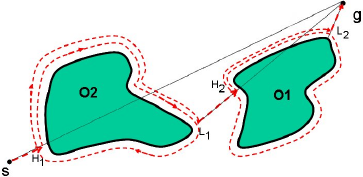
\includegraphics[scale=0.7]{./algorytmy/Bug1}
	\caption{ Bezkolizyjna ścieżka wyznaczona przez algorytm Bug }\label{fig:Bug1}
	\end{figure}
	Ścieżka wyznaczona przez ten algorytm jest daleka od optymalnej. Robot niezależnie od wybranego kierunku
	omijania przeszkody musi ją okrążyć całkowicie. W pewnych sytuacjach całkowite okrążenie przeszkody jest niemożliwe. Na przykład jesli robot natrfi na ścianę.
	W takim przypadku algorytm zawodzi całkowicie.
	Efektywność algorytmu można poprawić sprawdzając podczas okrążania przeszkody czy punkt w którym aktualnie
	znajduje  się robot jest poszukiwanym punktem położonym najbliżej celu. Przykładowa ścieżka
	wyznaczona za pomocą zmodyfikowanej wersji algorytmu jest widoczna na rysunku \ref{fig:Bug2}.
	Robot otacza przeszkodę w wybranym wcześniej kierunku i odłącza się od niej w momencie przecięcia
 	prostej łączącej punkt startowy z punktem docelowym. Uzyskana w ten sposób ścieżka nadal zależy od wybranego
	 a~priori kierunku jazdy.	
	\begin{figure}
	\centering
	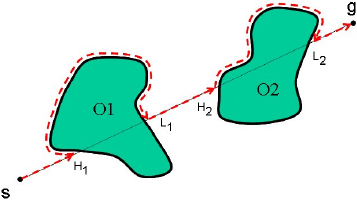
\includegraphics[scale=0.7]{./algorytmy/Bug2}
	\caption{Zasada działania algorytmu Bug w wersji rozszerzonej}\label{fig:Bug2}
	\end{figure}
	Obie zaprezentowane wersje algorytmu Bug nie uwzględniają ograniczeń wynikających z kinematyki robota, a w
	szczególności faktu, że rozpatrywany robot może być nieholonomiczny.
\subsection{Algorytm VHF}
	Pełna  anglojęzyczna nazwa metody brzmi \mbox{ \emph{Vector Field Histogram}}. Na język polski można ją
	przetłumaczyć jako algorytm histogramu pola wektorowego. Należy ona do grupy metod, które w czasie
	rzeczywistym pozwalają na jednoczesne wykrywanie i omijanie przeszkód oraz kierowanie robota na cel.
	Algorytm ten został szczegółowo opisany w pracy inżynierskiej \cite{inzynierka}, więcej informacji można też znaleźć w publikacjach autorów (\cite{VFH_1} oraz \cite{VFH_2}).
	W skrócie, jego zasada działania opiera się na konstrukcji dwuwymiarowego opisu świata w postaci siatki. Każdemu elementowi siatki przypisany jest poziom ufności oddający prawdopodobieństwo
	z jakim w danym położeniu może pojawić się przeszkoda (rysunek \ref{fig:VFH_siatka}).
	\begin{figure}[H]
	\centering
	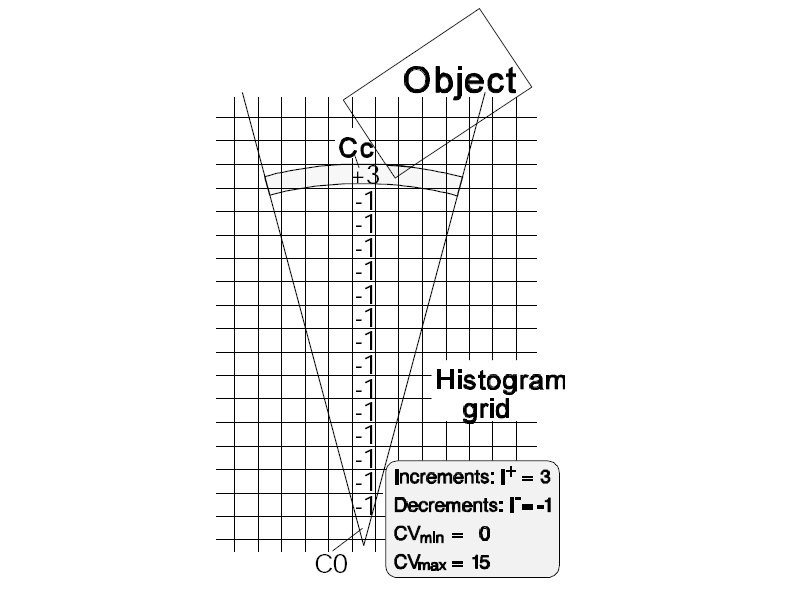
\includegraphics[scale=0.44]{./algorytmy/VFH_siatka}
	\caption{ Zasada tworzenia dwuwymiarowego histogramu \newline(na podstawie \cite{VFH_2})}\label{fig:VFH_siatka}
	\end{figure}
	Tak skonstruowana mapa redukowana jest do jednowymiarowego histogramu biegunowego (rysunek \ref{fig:VFH_hist_biegunowy}), który dodatkowo wygładzany jest przez
	filtr dolnoprzepustowy. W ten sposób otrzymuje się informację o poziomie ufności wystąpienia przeszkody poruszając się w danym kierunku (świadomie rezygnuje się z informacji o odległości od przeszkody).
	Na podstawie tego histogramu wyznaczane są sterowania dla robota. Histogram jest analizowany w poszukiwaniu minimów lokalnych, wszystkie doliny, których poziom ufności
	znajduje się poniżej ustalonego umownie progu są rozważane przy wyznaczaniu kierunku jazdy robota. Jeśli minimów jest kilka wybierane jest to, którego kierunek prowadzi najbliżej
	do celu. 
	Algorytm do poprawnego działania  potrzebuje informacji o rozłożeniu przeszkód w otoczeniu robota. W oryginalnej implementacji była ona pozyskiwana z sensorów ultradźwiękowych.
	Można je również zastąpić z powodzeniem czujnikami laserowymi. Obraz video z kamery umieszczonej nad eksplorowanym światem także dostarcza tej informacji (jak w rozgrywkach \emph{Small-size League}).
	\begin{figure}[H]
	\centering
	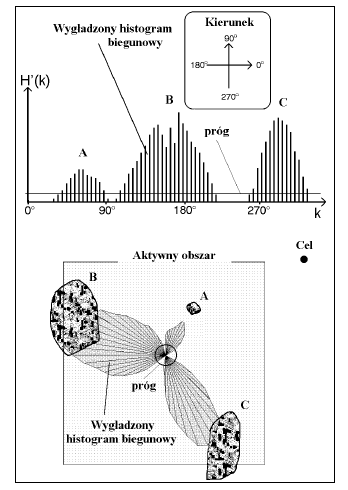
\includegraphics[scale=0.5]{./algorytmy/VFH_hist_biegunowy}
	\caption{ Histogram biegunowy dla przykładowego rozmieszczenia przeszkód \newline(na podstawie \cite{ISR})}\label{fig:VFH_hist_biegunowy}
	\end{figure}

	\subsection{Technika dynamicznego okna} \label{subsec:dynamic_window}
	Popularną, stosowaną w robotyce metodą unikania kolizji jest także technika dynamicznego okna. Algorytm ten analizuje jedynie możliwe do osiągnięcia w danej sytuacji prędkości.
	Więcej informacji na temat algorytmu można znaleźć w publikacji \cite{dynamic_window}.
	Ujmując w jednym zdaniu algorytm polega na przeszukiwaniu zbioru dopuszczalnych prędkości liniowych i kątowych, tak aby maksymalizować funkcję celu. Sposób konstrukcji funkcji celu
	gwarantuje, że wybrane prędkości będą prowadzić robota w zamierzonym kierunku oraz, że nie natrafi na przeszkodę.
\subsection{Algorytmy pól potencjałowych}
\subsubsection{Algorytm w wersji podstawowej}
	Kolejne podejście do problemu nawigacji robota mobilnego zaczerpnięto z fizyki. Problem znalezienia bezkolizyjnej ścieżki został sprowadzony do problemu konstrukcji
	funkcji opisującej rozkład energii w danym środowisku. W takim układzie dotarcie do celu jest równoważne ze znalezieniem minimum funkcji opisującej rozkład sztucznego pola
	potencjałowego. Robot podąża w kierunku ujemnego gradientu tej funkcji, mamy zatem $c(t)=- \nabla U(c(t))$. W klasycznym podejściu sztuczne pole potencjałowe tworzy
	się w ten sposób, że przeszkody są źródłem ujemnego pola(odpychającego), natomiast cel emituje pole dodatnie. Ujęte jest to w następujących wzorach:
	\begin{equation}
	U(q) = U_{att}(q) + U_{rep}(q)
	\end{equation}
	\begin{equation}\label{eq:U_att}
		U_{att}(q) = \left\{ 
		\begin{array}{l l}
		\frac{1}{2}\xi d^2 & \quad \mbox{dla $d\leqq d^{*}_{goal}$ }\\
		\xi d^{*}_{goal}d - \frac{1}{2}(d^{*}_{goal})^{2} & \quad \mbox{dla $d\geqq d^{*}_{goal}$ }\\
		\end{array} \right. 
	\end{equation}
	, gdzie $d=d(q,q_{goal})$ jest odległością danego położenia od celu, $\varepsilon$ jest stałą określającą poziom przyciągania do celu, natomiast $d^{*}_{goal}$ określa próg,
	po którym funkcja z kwadratowej przechodzi w trójkątną.
	Oddziaływanie przeszkód opisane jest następującym wzorem:
	\begin{equation}
		U_{rep}(q) = \left\{ 
		\begin{array}{l l}
		\frac{1}{2} \eta{ ( \frac{1}{D(q)} - \frac{1}{ Q^{*} } )}^2  & \quad \mbox{dla $D(q)\leq Q^{*} $ }\\
		0 & \quad \mbox{dla $D(q)> Q^{*}$ }\\
		\end{array} \right.
	\end{equation}
	,gdzie $ Q^{*} $ jest zasięgiem pola odpychającego przeszkody, natomiast $\eta$ odpowiada za siłę tego pola. 
	Kierunek, w którym podążać ma robot wyznaczany jest ze wzoru:
	\begin{equation}
	- \nabla U(q) = - \nabla U_{att}(q) - \nabla U_{rep}(q)
	\end{equation}
	Powyższe podejście w stosunkowo prosty sposób umożliwia wyznaczenie kierunku bezkolizyjnej ścieżki do celu. Posiada ono jednak pewną dość istotną wadę. Mianowicie w pewnych, 
	szczególnych sytuacjach robot może utknąć w minimum lokalnym. Sposób w jaki konstruowana jest funkcja celu w żaden sposób nie wyklucza występowania minimów lokalnych.
	W przypadku, gdy sterowany robot utknie w takim minimum, konieczna jest reakcja ze strony wyższej warstwy nawigującej maszyną. Przykładowo można wykorzystać algorytm 
	błądzenia losowego.
\subsubsection{Funkcja nawigacji}
	Istnieje jednak pewna szczególna funkcja, która posiada tylko globalne minimum, została ona zdefiniowana w publikacjach \cite{navi_func1} oraz \cite{navi_func2}.
	Przykładowy wykres funkcji nawigacji zamieszczony jest na rysunku ~\ref{fig:func_navi}. Zasięg oddziaływania minimum globalnego zależy od kilku istotnych parametrów, które zawarte są 
	we wzorze opisującym rozkład sztucznego potencjału.
	\begin{figure}[!h]
	\centering
	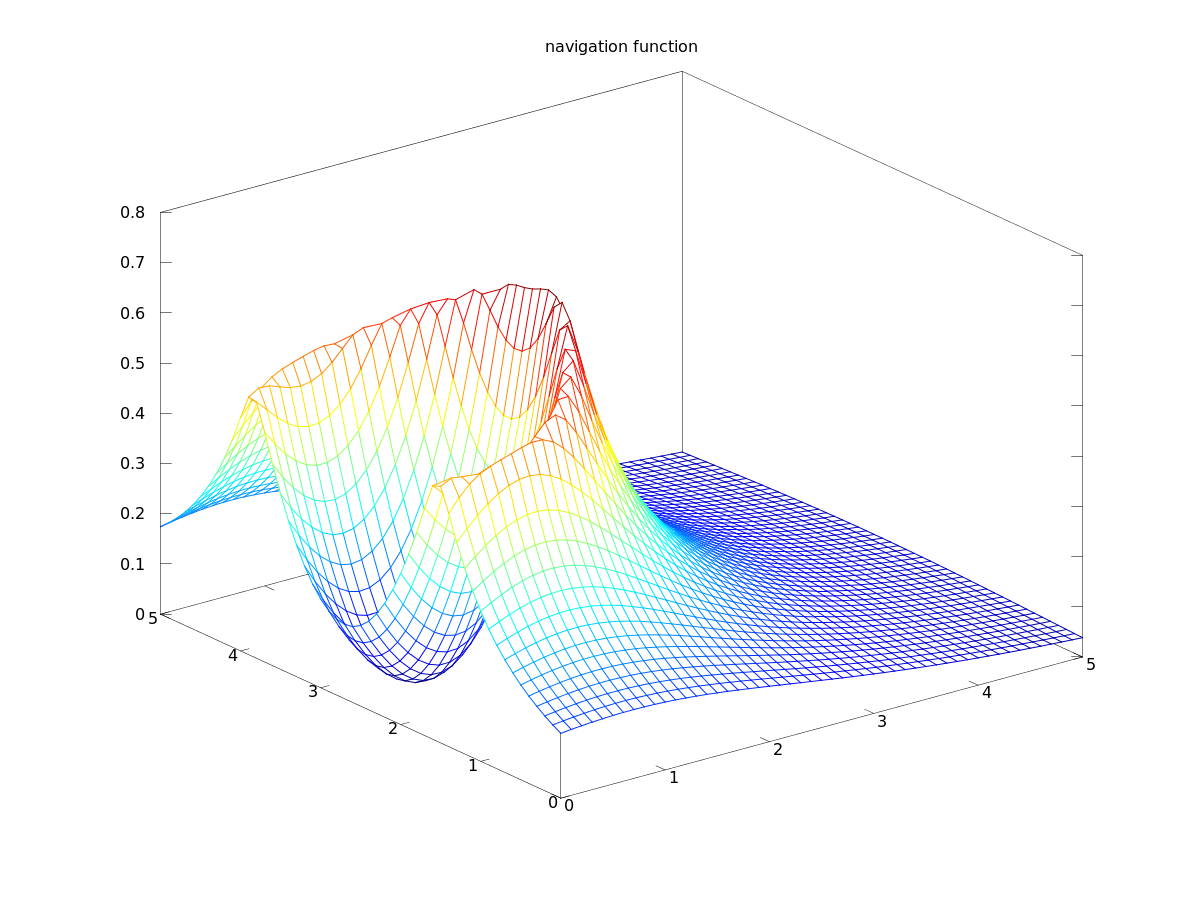
\includegraphics[scale=0.3]{./algorytmy/navigation_func_k_10}
	\caption{Funkcja nawigacji dla $\kappa=10$}
	\label{fig:func_navi}
	\end{figure}
	Dla bieżącego położenia robota $q$ funkcja nawigacji zdefiniowana jest następująco:
	\begin{equation}
	\label{eq:navi_func}
	\phi = \frac{(d(q,q_{goal}))^2}{ (\lambda \beta(q) + d(q,q_{goal})^{2\kappa} )^{\frac{1}{\kappa}}}
	\end{equation}
	gdzie $\beta(q)$ jest iloczynem funkcji odpychających zdefiniowanych dla wszystkich przeszkód:
	\begin{equation}
	\beta  \stackrel{ \vartriangle }{ = } \prod_{i=0}^{N}{ \beta_i(q)}    
	\end{equation}
	Natomiast dla każdej przeszkody($i>0$) funkcja określona jest następująco:
	\begin{equation}
	\beta_{i}(q)=(d(q,q_i))^2 - r_i^{2} \text{ dla i = 1...N, gdzie N jest liczbą przeszkód}
	\end{equation}
	Powyższą funkcję definiuje się dla każdej z przeszkód o promieniu $r_i$, której środek znajduje się w punkcie $q_i$.
	Jak łatwo zauważyć, funkcja ta przyjmuje ujemne wartości wewnątrz okręgu opisującego przeszkodę, natomiast dodatnie na zewnątrz okręgu.
	Dodatkowo definiuje się funkcję $\beta_{0}(q)= -(d(q,q_0))^{2} + r_0^{2}$, w której parametry $r_0$ oraz $q_0$ oznaczają odpowiednio promień świata w którym porusza się robot
	oraz środek tego świata.
	Wzór \ref{eq:navi_func} posiada dwa istotne parametry. Pierwszy z nich, $\lambda$ ogranicza przeciwdziedzinę do przedziału $[0,1]$, gdzie wartość $0$ jest tożsama z osiągnięciem celu, natomiast
	$1$ jest osiągana na brzegu każdej z przeszkód. Drugi parametr $\kappa$ odpowiednio dobrany powoduje, że blisko celu wykres funkcji $\phi$ przybiera kształt misy.
	Zwiększanie parametru $\kappa$ powoduje przesuwanie globalnego minimum w kierunku położenia punktu docelowego. Zwiększone jest zatem oddziaływanie przyciągającego pola emitowanego przez 
	punkt docelowy.

	Wykres funkcji nawigacji przedstawiony na rysunku \ref{fig:func_navi} został sporządzony dla następujących parametrów (wszystkie jednostki wyrażone są w metrach):
	\begin{enumerate}
	\item eksplorowany świat ograniczony jest okręgiem o środku w punkcie $q_0(2.7;3.7)$ i promieniu $r_0 = 7.4$,
	\item $\lambda = 0.2$,
	\item $\kappa = 10$,
	\item przeszkody umiejscowione są w punktach $(2;2),(3;3)(4;4),(3.5;3.5)$ i mają stały promień, odpowiadający modelowi robota
	zastosowanemu podczas doświadczeń $r_i = 0.14 $,
	\item punkt docelowy ma współrzędne $q_g(2.7;0.675)$,
	\item funkcja nawigacji została wykreślona z krokiem $0.1$.
	\end{enumerate}

\subsection{Algorytm CVM (\textit{Curvature Velocity Method})}
	W pracy inżynierskiej \cite{inzynierka} jako docelowy algorytm unikania kolizji wybrany został właśnie \texttt{CVM}.
	Metoda krzywizn i prędkości (ang. \textit{Curvature Velocity Method}) została zaproponowana przez R. Simmonsa w
	\cite{CVM_2}, należy do grupy metod bazujących na przeszukiwaniu przestrzeni prędkości, a jej działanie
	jest zbliżone do techniki dynamicznego okna zaprezentowanej w \ref{subsec:dynamic_window}.

	Spośród wszystkich par $(v,\omega)$ wybierana jest taka, która osiąga największą wartość funkcji celu.
	Podejście takie umożliwia uwzględnienie przede wszystkim ograniczeń kinematycznych, ale także i dynamicznych.
	Wyznaczone przez algorytm sterowanie na następny krok definiuje łuk $c=\frac{\omega}{v}$, po którym będzie
	poruszał się robot do chwili wyznaczenia kolejnego sterowania.
	
	Funkcja celu została tak skonstruowana, aby preferować prędkości, które prowadzą do celu, ale jednocześnie  
	nie powodują kolizji. Ponadto dołożone zostało kryterium na maksymalizację prędkości liniowej robota. Funkcja celu jest zatem sumą ważoną trzech składowych: 
	\begin{equation} \label{eq:fcelu_cvm}
	F(v,\omega)=\alpha_1 \mathcal{V}(v,\omega)+\alpha_2 \mathcal{D}(v,\omega) + \alpha_3 \mathcal{G} (v,\omega))
	\end{equation}
	gdzie:
	\begin{itemize}
	 \item $\alpha_1, \alpha_2, \alpha_3$ współczynniki wagowe,
	 \item funkcja $\mathcal{V}(v,\omega)$ określa stosunek między ocenianą prędkością liniową a maksymalną,
	 \item funkcja $\mathcal{D}(v,\omega)$ określa odległość od najbliższej przeszkody na którą napotka robot poruszający się po trajektorii wyznaczonej przez $(v,\omega)$,
	 \item funkcja $\mathcal{G}(v,\omega)$ odpowiada za kierowanie się robota na cel.
	\end{itemize}
	Zachowaniem robota można sterować poprzez zmianę wartości współczynników wagowych. W skrajnych przypadkach,
	gdy któryś ze współczynników zostanie wyzerowany, traci on całkowicie wpływ na trajektorię po której
	porusza się robot. Szczegółowy opis poszczególnych składowych, jak i samego działania metody został
	zaprezentowany w paragrafie \ref{sec:CVM:action}.

	\section{Zasada działania CVM \label{sec:CVM:action}} 
	Omawianie mechanizmu wyboru najlepszego sterowania z wykorzystaniem algorytmu \textit{CVM} należy rozpocząć od przypomnienia funkcji celu (\ref{eq:fcelu_cvm})
	\begin{equation*}
	F(v,\omega)=\alpha_1 \mathcal{V}(v,\omega)+\alpha_2 \mathcal{D}(v,\omega) + \alpha_3 \mathcal{G} (v,\omega))
	\end{equation*}
	W powyższym równaniu składowe odpowiadające za kierowanie na cel oraz za maksymalizację prędkości liniowej zostały zdefiniowane następująco:
	\begin{gather}
	\mathcal{V}(v,\omega)=\frac{v}{V_{max}} \label{eq:CVM_speed}\\
	\mathcal{G}(v,\omega)=1-\frac{|\theta_{cel} -T_{alg}\omega|}{\pi} \label{eq:CVM_head}
	\end{gather}
	gdzie:
	\begin{itemize}
	 \item $V_{max}$ -- maksymalna prędkość liniowa z jaką może poruszać się robot
	 \item $T_{alg}$ -- czas na jaki wystawiane jest obliczone sterowanie
	 \item $\theta_{cel}$ -- orientacja do celu w układzie współrzędnych robota 
	\end{itemize}
	Natomiast zdefiniowanie składowej odpowiedzialnej za omijanie przeszkód wymaga określenia pewnych dodatkowych 
	funkcji wykorzystywanych w algorytmie. Należy dokonać przekształcenia opisu przeszkód we współrzędnych
	kartezjańskich  do przestrzeni prędkości. Dokonywane jest to za pomocą odległości do punktu $p$, w którym wystąpi kolizja z przeszkodą  $o$, jeśli robot będzie poruszał się po trajektorii $c=\frac{\omega}{v}$. Wartość ta jest oznaczana jako
	$d_c((0,0),p)$, gdzie $p$ jest punktem zderzenia z przeszkodą.
	Następnie należy zdefiniować funkcję odległości robota od przeszkody:
 	\begin{equation}\label{eq:CVM_dv}
	d_v(v,\omega,p)= \left\{ 
	\begin{array}{l l}
  	d_c((0,0),p_i & \quad \mbox{dla $v\neq0$}\\
  	\infty & \quad \mbox{dla $v=0$ }\\
	\end{array} \right. 
	\end{equation}
	Dla danego zbioru przeszkód $O$ zawsze wybierana jest odległość do najbliższej przeszkody leżącej na trajektorii. Zatem funkcję dla danego zbioru przeszkód $O$ można zapisać następująco:
 	\begin{equation}\label{eq:CVM_Dv2}
	D_v(v,\omega,O)= \underset{o \in O}{\operatorname{inf}} d_v(v,\omega,o)
	\end{equation}
	W rzeczywistości jednak informacja o położeniu przeszkód jest ograniczona do pewnego obszaru, który może
	wynikać z zasięgu czujników w jakie wyposażony jest robot, bądź ze sztucznego ograniczenia zasięgu działania
	algorytmu w przypadku, gdy możliwy jest dostęp do globalnej informacji o położeniu przeszkód. Zasięg algorytmu  będzie  w dalszej część pracy oznaczany jako $L$. Funkcja  (\ref{eq:CVM_Dv})
	jest zatem ograniczona od góry w sposób następujący:
 	\begin{equation}\label{eq:CVM_Dv_ogr}
	D_{ogr}(v,\omega,P)= \min(L, D(v,\omega,P))
	\end{equation}
	Po uprzednim zdefiniowaniu niezbędnych funkcji  można podać postać funkcyjną składowej funkcji celu odpowiadającej za unikanie kolizji:
	\begin{equation} \label{eq:CVM_dist}
	\mathcal{D}(v,\omega)=\frac{D_{ogr}}{L}
	\end{equation}
 	
	Aby sposób obliczania odległości do przeszkody był możliwie jak najprostszy, każda przeszkoda jest
	reprezentowana w algorytmie jako okrąg o  promieniu \emph{r} (wynikającym z jej rozmiarów) i współrzędnych środka $(x_0,y_0)$. Można zatem dość łatwo wyznaczyć odległość, jaką przebędzie robot poruszający się po łuku wyznaczonym przez parę $(v,\omega)$ do
	momentu przecięcia z okręgiem. Zostało to zobrazowane na rysunku \ref{fig:CVM_dist}.
	\begin{figure}[!b]
	\centering
	%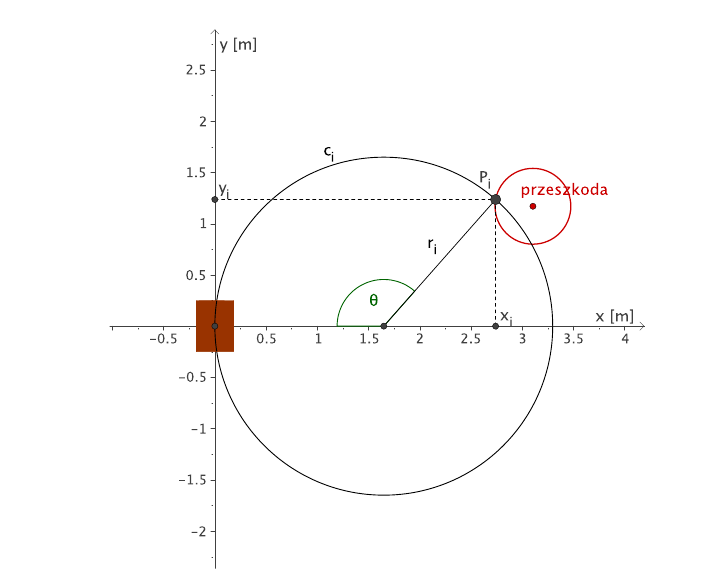
\includegraphics[scale=0.43]{./algorytmy/CVM_dist}
	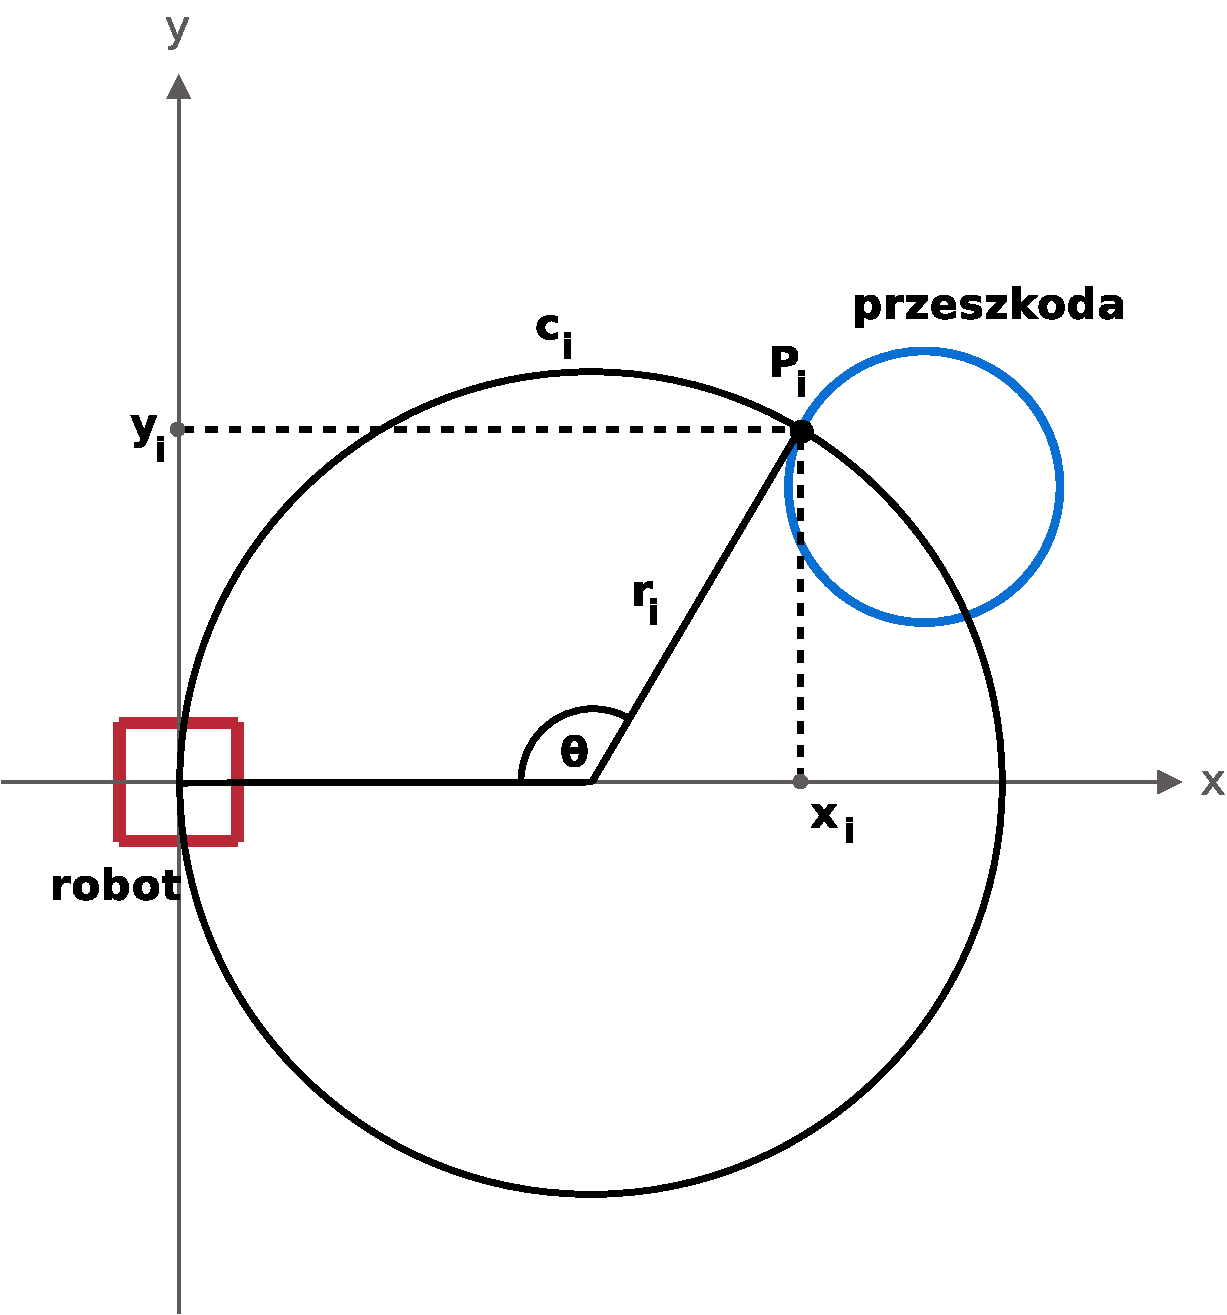
\includegraphics[scale=0.35]{./algorytmy/CVM_dist_new}
	\caption{ Obliczanie odległości od przeszkody \label{fig:CVM_dist}}
	\end{figure}
	
	Dla robota o początkowej orientacji zgodnej z osią $OY$, poruszającego się po trajektorii o krzywiźnie $c$ przecinającej
	okrąg opisujący przeszkodę w punkcie $P(x,y)$ prawdziwe są następujące wzory:
	\begin{equation}\label{eq:CVM_teta}
	\theta= \left\{ 
	\begin{array}{l l}
	\text{atan2}(y,x-\frac{1}{c} )& \quad \mbox{dla $c<0$}\\
  	\pi-\text{atan2}(y,x-\frac{1}{c}) & \quad \mbox{dla $c>0$}\\
	\end{array} \right. 
	\end{equation}
	
	\begin{equation}
	d_c((0,0),P)= \left\{ 
	\begin{array}{l l}
  	y& \quad \mbox{dla $c=0$}\\
  	|\frac{1}{c}|\theta & \quad \mbox{dla $c\neq0$}\\
	\end{array} \right. 
	\end{equation}
	Zastosowana we wzorze (\ref{eq:CVM_teta}) funkcja \emph{atan2} zwraca wartości z przedziału $[-\pi;\pi]$, zatem uwzględnia w której ćwiartce leży kąt:
	\begin{equation}\label{eq:atan2}
	\text{atan2}(y,x)= \left\{ 
	\begin{array}{l l}
	\arctan{\frac{|y|}{|x|}} \sgn{(y)} & \quad \mbox{dla $x>0$}\\
	\frac{\pi}{2}\sgn{(y)} & \quad \mbox{dla $x=0$}\\
	\pi-\arctan{\frac{|y|}{|x|}} \sgn{(y)} & \quad \mbox{dla $x<0$}\\
	\end{array} \right. 
	\end{equation}
	
	Jednakże obliczanie odległości od przeszkody dla każdego sterowania $(v,\omega)$ w sposób omówiony powyżej
	jest czasochłonne. Stąd konieczne jest kolejne uproszczenie. Łatwo zauważyć, że z punktu $(0,0)$ w którym
	znajduje się robot można poprowadzić dwa łuki styczne do okręgu opisującego przeszkodę $p$. Zatem na zewnątrz
	krzywych stycznych odległość  $d_c((0,0),p)$ jest nieskończona. Natomiast dla krzywizn zawierających się
	pomiędzy łukami stycznymi można dokonać przybliżenia wartością stałą. Omawiana sytuacja została zobrazowana na
	rysunku \ref{fig:CVM_styczne}.
	\begin{figure}[!b]
	\centering
	%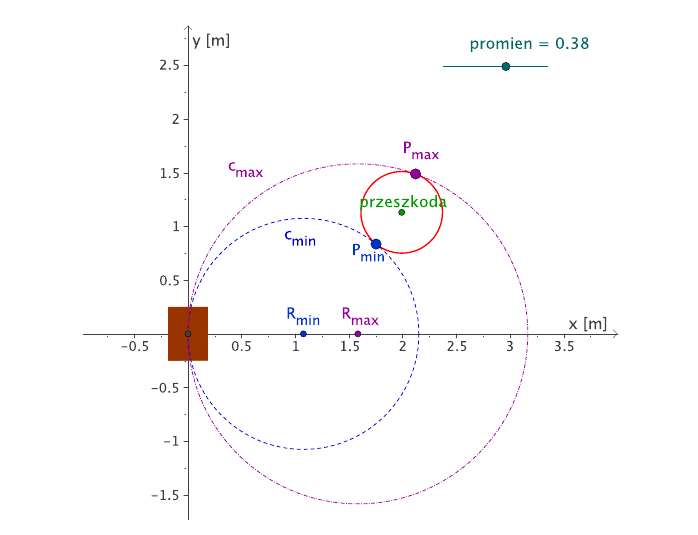
\includegraphics[scale=0.45]{./algorytmy/CVM_styczne}
	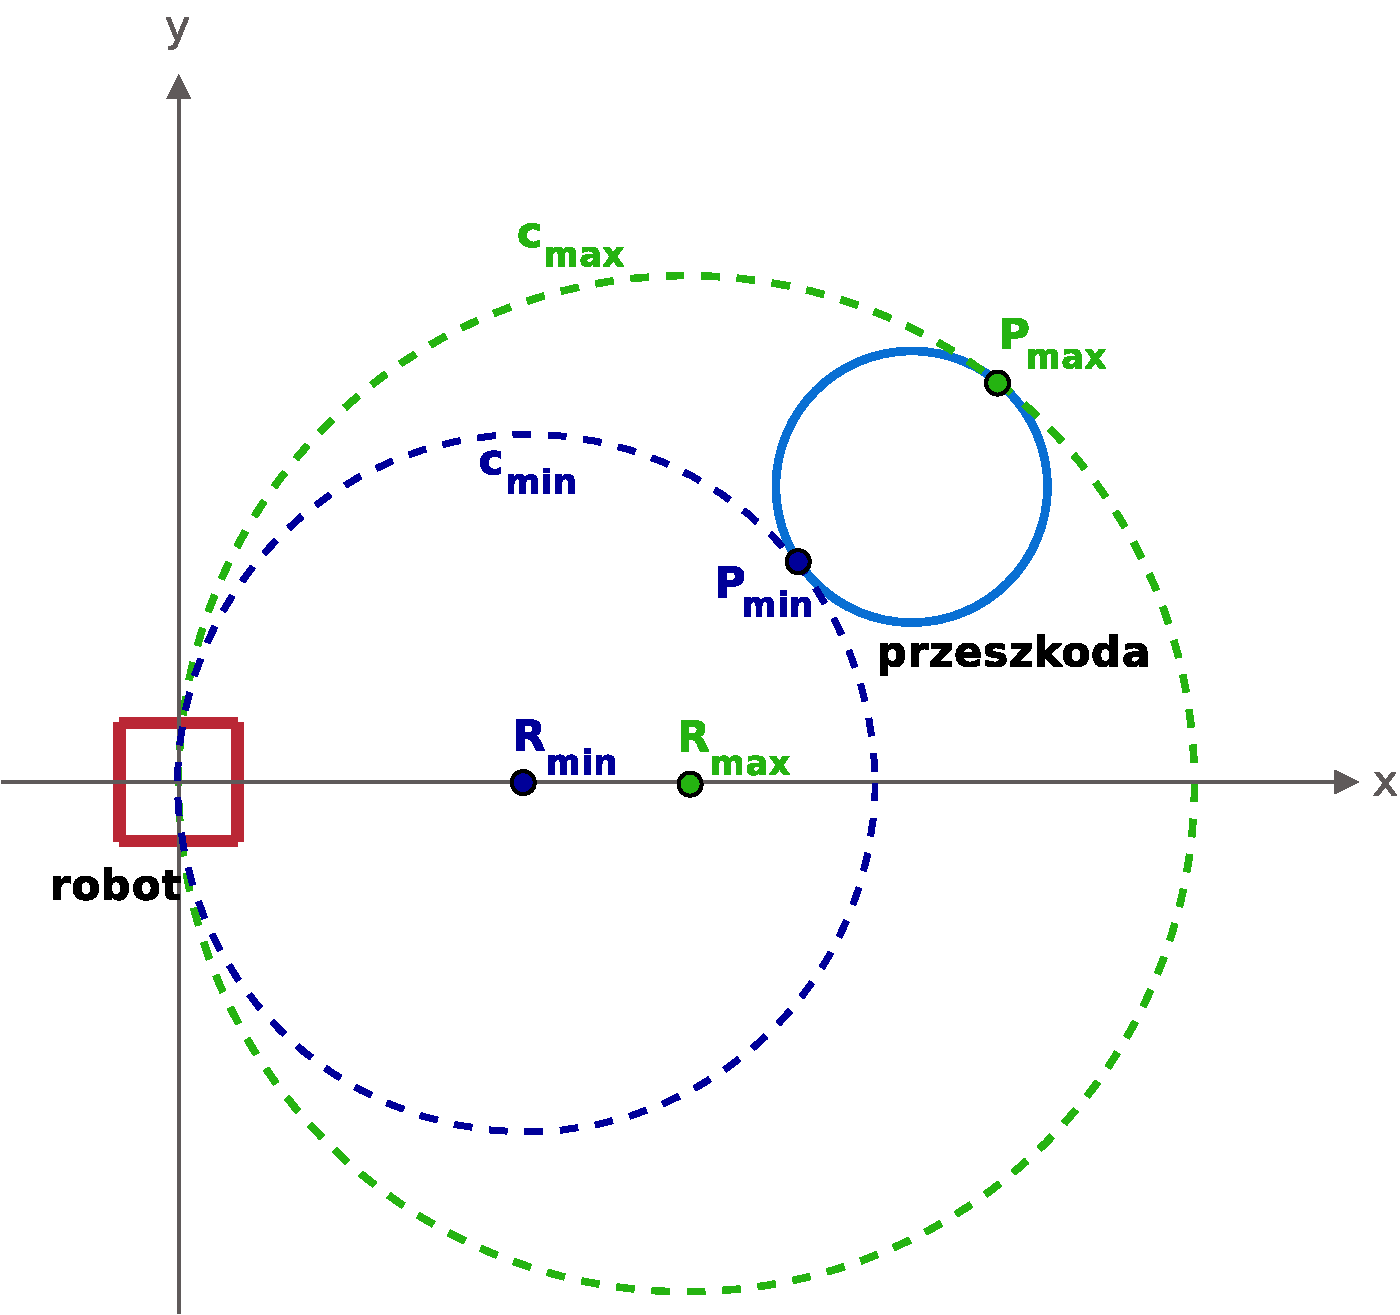
\includegraphics[scale=0.32]{./algorytmy/CVM_styczne_new}
	\caption{ Zasada wyznaczania przedziału $(c_{min}$,$c_{max})$ \label{fig:CVM_styczne}}
	\end{figure}
	Aby wyznaczyć okręgi styczne do okręgu opisującego przeszkodę należy znaleźć takie $r$ dla którego
	poniższy układ równań ma dokładnie jedno rozwiązanie:
	\begin{equation}\label{eq:CVM_styczne}
	 \left\{ 
	\begin{array}{l l}
  	(x-x_0)^2 + (y-y_0)^2={r_0}^2\\
  	 (x-r)^2 + y^2={r}^2\\
	\end{array} \right. 
	\end{equation}
	Gdzie $(x_0,y_0)$ jest środkiem okręgu opisującego przeszkodę, natomiast $r_0$ jego promieniem.
	W wyniku takiego postępowania można otrzymać punkty styczności $P_{max}$ oraz $P_{min}$ oraz odpowiadające im krzywizny $c_{min}$ oraz $c_{max}$. 
	Ostatecznie można już dokonać przybliżenia odległości po łuku od rozpatrywanej przeszkody $p$ w następujący sposób:
	\begin{equation}\label{eq:CVM_dv_const}
	d_v(v,\omega,p)= \left\{ 
	\begin{array}{l l}
  	\min(d_c((0,0),P_{max}),d_c((0,0),P_{min})) & \quad \mbox{$c_{min}\leq c \leq c_{max}$  }\\
  	\infty & \quad \mbox{w p.p. }\\
	\end{array} \right. 
	\end{equation}

	Zaprezentowane rozumowanie prowadzi do sytuacji, w której zbiorowi przeszkód $O$ odpowiada zbiór przedziałów krzywizn o stałej odległości od przeszkody. W dalszej części pracy przedział będzie rozumiany jako trójka liczb postaci $([c_1,c_2],d_{1,2})$, gdzie $c_1$,$c_2$ to krzywizny okręgów wyznaczających ten przedział, natomiast $d_{1,2}$ jest odległością zdefiniowaną równaniem (\ref{eq:CVM_dv_const}).
	
	Ze zbioru przedziałów należy następnie utworzyć listę przedziałów $\mathbb{S}$, tak, aby zawierała
	przedziały $s$ rozłączne o odległości do najbliższej przeszkody (zgodnie z równaniem (\ref{eq:CVM_Dv})).
	W oryginalnej pracy na temat \textit{CVM} \cite{CVM_2} zaproponowany został algorytm (\ref{alg:CVM_lista}) realizujący to zadanie.

	\begin{algorithm}
	\caption{tworzy listę rozłącznych przedziałów $\mathbb{S}$}
	\label{alg:CVM_lista}
	\begin{algorithmic}
	\STATE $ \mathbb{S}:= ((-\infty;\infty),L) $
	\STATE  wybierz kolejny nie dodany przedział $([c_{min};c_{max}],d)$
	\FORALL {$ s\in \mathbb{S}$}
	\IF {zbiory są rozłączne } 
	\STATE nic nie rób
	\ELSIF {s zawiera się w $([c_{min};c_{max}],d)$}
	\STATE ustaw odległość $s.d= min(s.d,d) $
	\ELSIF {s zawiera  $([c_{min};c_{max}],d)$}
		\IF{$d<s.d$}
		\STATE podziel $s$ na trzy przedziały: \\$([s.c_{min};c_{min}],s.d)$, $([c_{min};c_{max}],d)$, $([c_{max};s.c_{max}],s.d)$ 
		\ELSE
		\STATE nic nie rób
		\ENDIF
	\ELSIF {s częściowo zawiera $([c_{min};c_{max}],d)$ }
		\IF{$d<s.d$}
		\STATE podziel $s$ na dwa przedziały
			\IF{$c_{max} > s.c_{max}$}
			\STATE podziel na przedziały $([s.c_{min};c_{min}],s.d)$ $([c_{min};s.c_{max}],d)$
			\ELSE
			\STATE podziel przedziały $([s.c_{min};c_{max}],d)$ $([c_{max};s.c_{max}],s.d)$
			\ENDIF
		\ELSE
		\STATE nic nie rób
		\ENDIF
	\ENDIF
	\ENDFOR
	\end{algorithmic}
	\end{algorithm}

	W zależności od rozmieszczenia przeszkód w środowisku przedziały wyznaczone przez krzywizny $c_{min}$ oraz $c_{max}$ charakteryzują się różną szerokością. Często przybliżenie zbioru długości krzywych należących do
	$[c_{min},c_{max}]$ jedną stałą wartością jest niewystarczające. Zazwyczaj przedział ten zawiera zbiór łuków których odległość od przeszkody jest istotnie mniejsza niż ta wynikająca ze wzoru (\ref{eq:CVM_dv_const}). Sytuacja taka została zilustrowana na rysunku \ref{fig:CVM_segmentacja}.
	\begin{figure}[!t]
	\centering
	%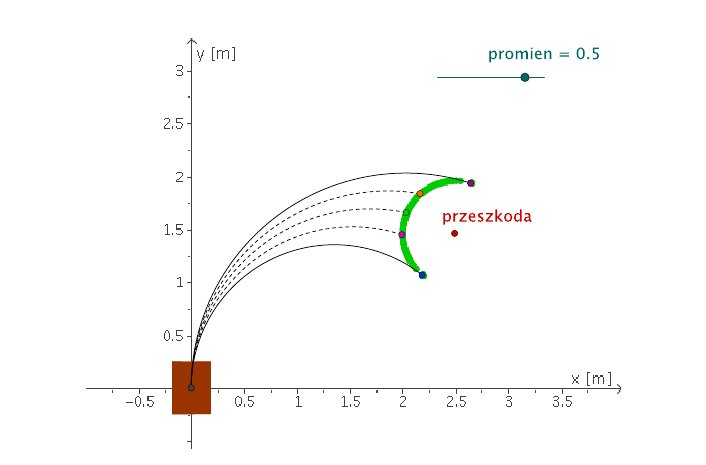
\includegraphics[scale=0.45]{./algorytmy/CVM_segmentacja}
	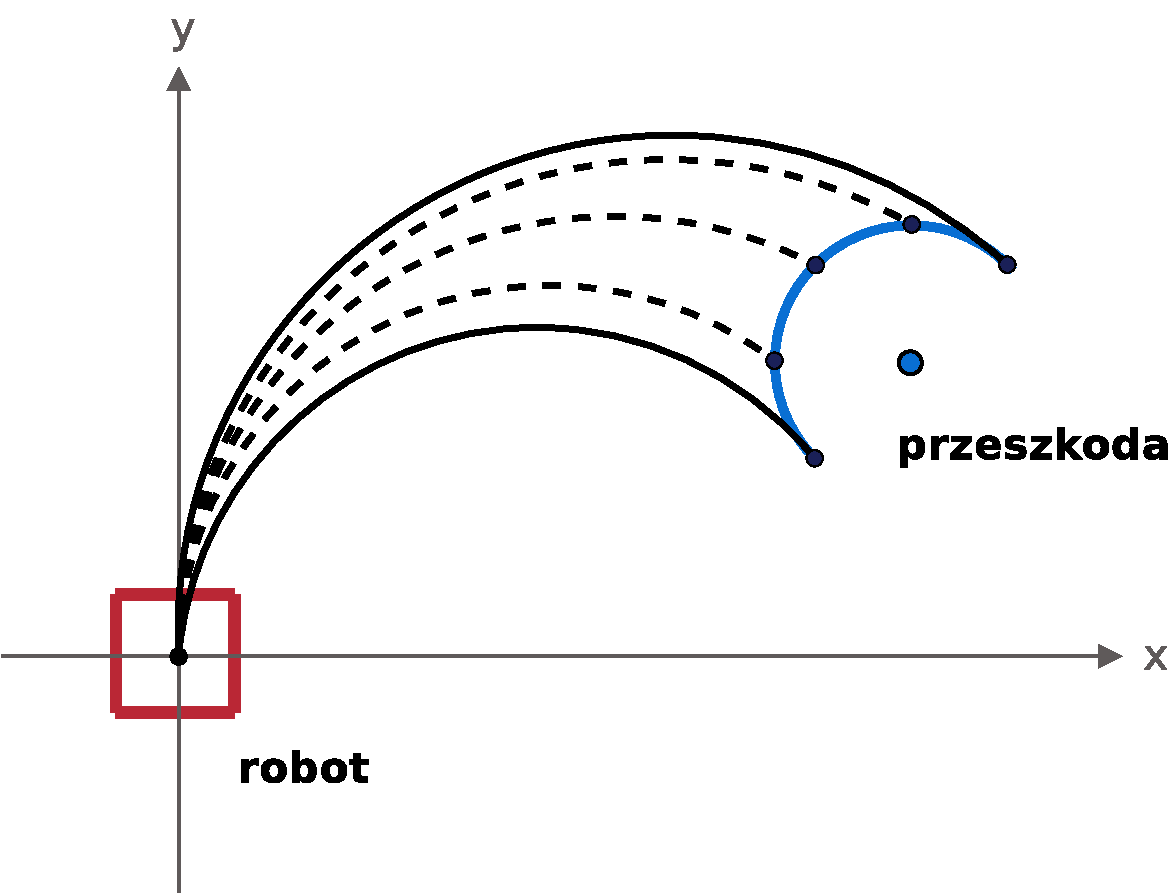
\includegraphics[scale=0.40]{./algorytmy/CVM_segmentacja_new}
	\caption{ Ukazanie sensu zastosowania segmentacji} \label{fig:CVM_segmentacja}
	\end{figure}

	Jednym z możliwych rozwiązań powyższego problemu jest podzielenie przedziału $[c_{min},c_{max}]$ na kilka
	pod przedziałów i do każdego z nich zastosowanie równania (\ref{eq:CVM_dv_const}) w celu wyznaczenia odległości od przeszkody. W pracy przyjęto rozwiązanie analogiczne jak opisane w \cite{majchrowski}.
	Pierwszym etapem jest wyznaczenie punktu leżącego na okręgu reprezentującym przeszkodę położonego najbliżej robota zgodnie z  metryką euklidesową. Następnie okrąg jest dzielony symetrycznie na $k$  segmentów. Postępowanie takie zostało przedstawione na rysunku \ref{fig:CVM_segmentacja2}. 
	Dla każdych dwóch sąsiadujących ze sobą punktów leżących pomiędzy punktami styczności $P_{min}$ oraz $P_{max}$
 	wyznaczane są krzywizny $c_1$ oraz $c_2$ i tworzony jest przedział. Jako odległość przyjmowana jest krótsza 
	z odległości zgodnie ze wzorem (\ref{eq:CVM_dv_const}). Tak otrzymane przedziały są dodawane do listy za pomocą algorytmu \ref{alg:CVM_lista}.
	
	\begin{figure}[H]
	\centering
	%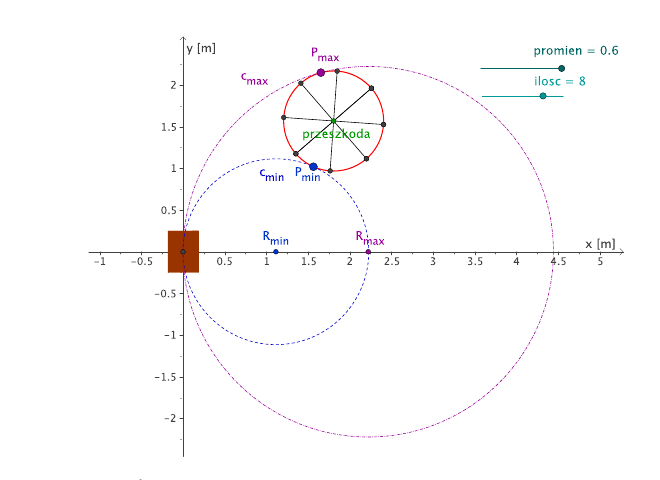
\includegraphics[scale=0.40]{./algorytmy/CVM_segmentacja2}
	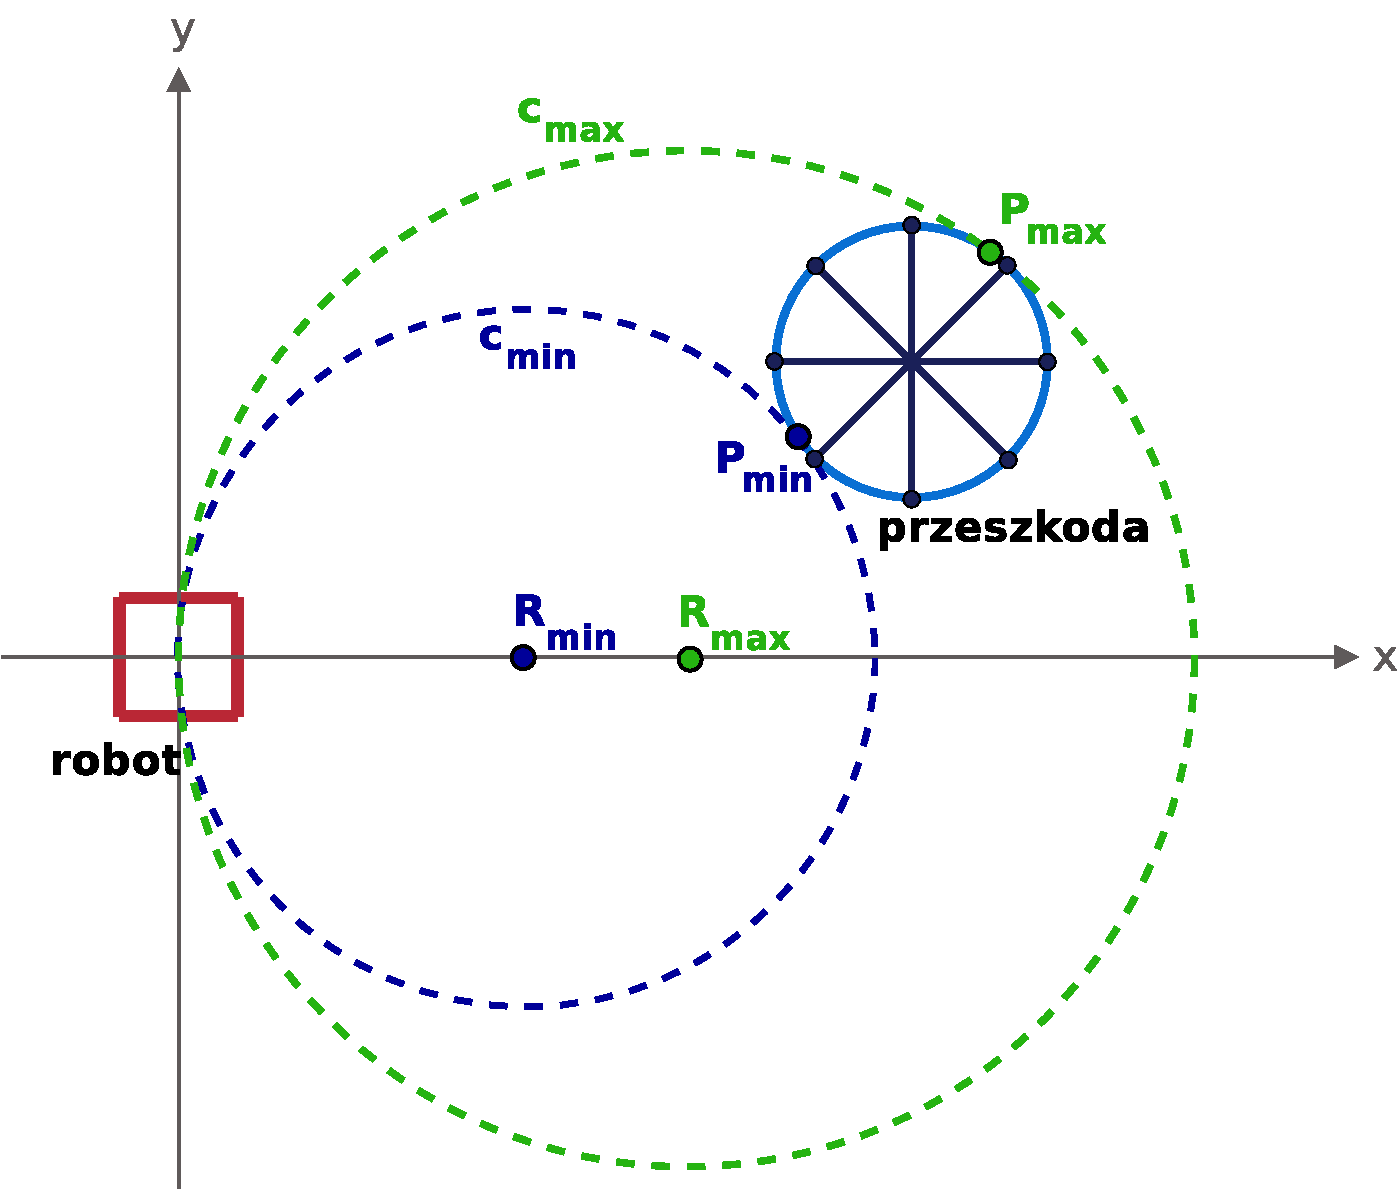
\includegraphics[scale=0.34]{./algorytmy/CVM_segmentacja2_new}
	\caption{ Efekt podziału okręgu na części} \label{fig:CVM_segmentacja2}
	\end{figure} 
\section{Algorytm RRT\\(\textit{Rapidly-Exploring Random Tree}) \label{sec:RRT:basic}}
Kolejnym zupełnie odmiennym podejściem w planowaniu bezkolizyjnej ścieżki jest losowe przeszukiwanie dopuszczalnej przestrzeni położeń robota. Szczegółowe informacje na
jego temat można znaleźć w \cite{RRT} oraz w \cite{RRT2}.
Algorytm RRT jest wydajnym algorytmem, który w czasie rzeczywistym może wyznaczyć drogę do celu, jednak nie jest ona optymalna pod względem dynamiki, kinematyki ani długości.
Podstawową strukturą danych na której operuje algorytm jest drzewo. Jako korzeń przyjmowany jest stan reprezentujący położenie robota w momencie uruchomienia algorytmu.
Budowa drzewa polega na dodawaniu kolejnych węzłów do drzewa w kierunku punktu obranego w danym kroku jako docelowy. Tymczasowy stan docelowy generowany jest w następujący sposób:
 \begin{algorithm}[H]
	
	\caption{ Funkcja obliczająca stan docelowy }
	\label{alg:chooseTarget}
	\begin{algorithmic}
	\STATE \texttt{function} \textit{chooseTarget}(\textit{goal:state}) \textit{state};
	\STATE p = \texttt{uniformRandom in}$[0.0 ...1.0]$
	\IF{$0.0<p<goalProb$} 
	  \RETURN  \texttt{goal};
	\ELSIF{ $goalProb<p<1.0$}
	  \RETURN \textit{RandomState()}
	\ENDIF
	\end{algorithmic}
  \end{algorithm}

Na listingu \ref{alg:chooseTarget} użyta została funkcja \texttt{RandomState}, zwracająca losowy punkt ze zbioru wszystkich możliwych położeń robota.
W najprostszej realizacji, może ona zwracać współrzędne punktu dobierane z rozkładem jednostajnym z określonego przedziału.
W każdej iteracji algorytmu tymczasowy stan docelowy obliczany jest na nowo. Aktualne drzewo, na którym operuje algorytm przeszukiwane jest w celu znalezienia
węzła \texttt{nearest} położonego najbliżej tego celu. Węzeł \texttt{nearest} rozszerzany jest w kierunku tegoż celu za pomocą funkcji \texttt{extend}.
Operacja ta w najprostszym ujęciu polega na stworzeniu nowego węzła przesuniętego względem \texttt{nearest} o odcinek \texttt{rrtStep} w kierunku tymczasowego celu.
Istotne jest, aby sprawdzić czy nowo wygenerowany stan znajduje się w dopuszczalnej przestrzeni stanów \textdollar. W najprostszym wariancie można zastosować
heurystykę, sprawdzającą jedynie czy położenie to nie koliduje z żadną z przeszkód znajdujących się w danej sytuacji oraz czy robot jest w stanie do niego dotrzeć.
Bardziej zaawansowane heurystyki powinny sprawdzać czy na przykład podczas przemieszczania  się do nowej pozycji nie nastąpi kolizja z dynamiczną przeszkodą.
W ogólnym ujęciu algorytm \texttt{RRT} wygląda zatem następująco:
  \begin{algorithm}[H]
	\caption{ Ogólna zasada algorytmu \texttt{RRT} }
	\label{alg:RRT}
	\begin{algorithmic}
	\STATE zbuduj model eksplorowanego świata $\mapsto$ \texttt{env:environment};
	\STATE zainicjuj stan początkowy $\mapsto$ \texttt{initState:state};
	\STATE zainicjuj stan końcowy $\mapsto$ \texttt{goalState:state};
	\STATE
	\WHILE { \texttt{goalState.distance(nextState)} $>$ \texttt{minimalDistance} }
	  \STATE wybierz tymczasowy cel: \texttt{target} =  \texttt{chooseTarget(goalState)}
	  \STATE nearestState $=$ \texttt{ nearest(tree, target) }
	  \STATE \texttt{extendedState} $=$ \texttt{extend(env, nearest, target)}
	  \IF { \texttt{extendedState} $!=$ \texttt{NULL} } 
	    \STATE \texttt{addNode(tree, extended)}
	  \ENDIF
	\ENDWHILE
	\RETURN  \texttt{tree};
	\end{algorithmic}
  \end{algorithm}
W opisie algorytmu \ref{alg:RRT} użyte zostały nie omówione jeszcze funkcje, \texttt{distance} zwracająca odległość w sensie euklidesowym między dwoma węzłami drzewa,
\texttt{addNode} dodająca węzeł do bieżącego drzewa. Parametr \texttt{rrtStep} jest natomiast wyrażony w metrach.
Tak zaimplementowana wersja algorytmu może być zastosowana jako skuteczne narzędzie do bezkolizyjnej nawigacji robotem, jednak jego wydajność można poprawić poprzez
modyfikacje opisane w kolejnym podrozdziale.

\subsection{Modyfikacje algorytmu, czyli przejście z RRT do ERRT \label{sec:RRT:extend} }
Omawiany algorytm można zmodyfikować pod kątem szybkości działania. Po pierwsze, elementy drzewa można przechowywać w strukturach ułatwiających przeszukiwanie drzewa.
W literaturze stosowane są w tym celu \texttt{KD-drzewa}. Kolejną modyfikacją jest zapamiętywanie losowo wybranych węzłów ze ścieżki znalezionej w poprzednim uruchomieniu
algorytmu. W takim wariancie tymczasowy punkt docelowy obierany jest następująco:
 \begin{algorithm}[H]
	\caption{ Zmodyfikowana funkcja obliczająca stan docelowy }
	\label{alg:chooseTargetExt}
	\begin{algorithmic}
	\STATE \texttt{function} \textit{chooseTargetExt}(\textit{goal:state}) \textit{state};
	\STATE p = \texttt{uniformRandom in}$[0.0 ...1.0]$
	\STATE i = \texttt{uniformRandom in}$[0 ...number\_of\_waypoints -1]$
	\IF{$0.0<p<goalProb$} 
	  \RETURN  \texttt{goal};
	\ELSIF{ $goalProb<p<goalProb+wayPointProb$}
	  \RETURN \textit{WayPoints[i]}
	\ELSIF{ $goalProb+wayPointProb<p<1.0$}
	  \RETURN \textit{RandomState()}
	\ENDIF
	\end{algorithmic}
  \end{algorithm}
W publikacji \cite{RRT} prawdopodobieństwo podążania do właściwego celu ostatecznie ustalane zostało na poziomie $0.1$, natomiast \texttt{wayPointProb} wynosiło $0.7$.
\begin{figure}[h]
\centering
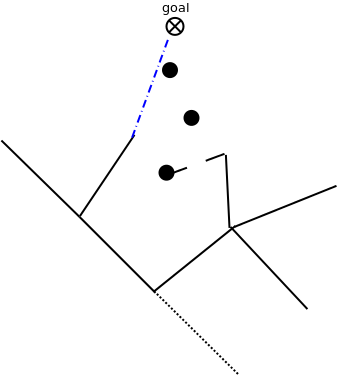
\includegraphics[scale=0.34]{./algorytmy/tree_with_waypoints.png}
\caption{ \texttt{RRT} z zapamiętanymi węzłami z poprzedniego uruchomienia. Linią kropkowaną zaznaczono gałąź dodaną w kierunku losowego punktu,
 linią przerywaną w kierunku jednego z elementów z poprzedniej ścieżki, a linią niebieską w kierunku celu.} \label{fig:tree_with_waypoints}
\end{figure} 
Kolejną modyfikacją jest zmiana sposobu obliczania odległości, standardowo w algorytmie wykorzystywana jest odległość pomiędzy liściem drzewa a punktem docelowym. Aby uniknąć
nadmiernego rozrastania drzewa, odległość może uwzględniać dodatkowo odległość liścia od korzenia pomnożoną przez określony współczynnik wagowy.

\section{Zalety algorytmu RRT w stosunku \\do CVM}
Podczas kontynuacji prac nad rozgrywkami RoboCup zdecydowano się na zmianę algorytmu wyznaczającego bezkolizyjną ścieżkę. Zmiana została wymuszona decyzją o zmianie
modelu sterowanego robota. Bazę jezdną o napędzie różnicowym zastąpiono holonomiczną. Algorytm CVM jest algorytmem dedykowanym do robotów o napędzie różnicowym, doskonale
można ująć w nim ograniczenia na dopuszczalne prędkości. Jednak sterowanie za jego pomocą robotem holonomicznym nie pozwala na pełne wykorzystanie możliwości robota.
Dodatkowo, jak zostało udowodnione w pracy inżynierskiej \cite{inzynierka}, CVM nie sprawdza się w silnie dynamicznym środowisku. Podczas testów z przeszkodami dynamicznymi osiągał
skuteczność na poziomie $80\%$. Kolizje występowały głównie w sytuacjach, kiedy przeszkoda uderzała w robota z boku lub z tyłu. Wynikało to z faktu, że trajektoria ruchu takiej przeszkody znajdowała się poniżej osi $OY$ w układzie współrzędnych
związanym ze sterowanym robotem. Przeszkody takiego typu nie były uwzględnianie przez algorytm.
RRT pozwala na uwzględnianie przeszkód rozsianych po całej planszy. Dodatkowo umożliwia poruszanie się po bardziej złożonych trajektoriach.
Kolejną zaletą RRT jest prostota w ograniczaniu przestrzeni, z której losowane są tymczasowe punkty docelowe. Dzięki temu w prosty sposób można ograniczyć poruszanie
się robota tylko do wnętrza boiska. w przypadku CVM istniała konieczność modelowania bandy boiska jako zbioru okręgów, mnożyło to ilość obiektów z jakimi należało detekować
kolizje.
Kolejnym problemem CVM jest nawigacja do celu znajdującego się za robotem, w pracy inżynierskiej wprowadzono modyfikację, zmieniającą parametr odpowiedzialny za kierowanie
robota na cel, uzależniając go od orientacji robota względem celu. Intencją było wymuszenie obrotu robota w kierunku celu, w sytuacji, gdy orientacja do celu jest duża.
Modyfikacja poprawiła skuteczność. Jednak nawet dla najlepszego zestawu współczynników wagowych wynosiła ona $80\%$. W przypadku bazy holonomicznej obracanie się w kierunku punktu docelowego nie jest
konieczne, stąd takie sterowanie nie jest optymalne.